\documentclass[11pt,letterpaper]{article}


\usepackage[numbers,square]{natbib}
\renewcommand\cite[1]{(\citet{#1})}
\usepackage[hmargin=0.75in]{geometry}
\usepackage{color}
\usepackage{chemarr}
\usepackage{amssymb}
\usepackage{graphicx}
\usepackage{epstopdf}
\usepackage{caption}
\usepackage{subcaption}
\usepackage{placeins}
\usepackage{gensymb}
\usepackage{array}
%\usepackage{underscore}
\newcolumntype{L}{>{\arraybackslash}m{12cm}}

\title{IGFEM-Curves-2D: User Manual}
\author{Marcus Hwai Yik Tan }
\date{Created on January 22nd, 2016. Last revised on \today}
\begin{document}
\maketitle

\section{Objective}
This project calculates the temperature distribution in a 2D rectangular domain given a channel network embedded in the domain. The temperature is obtained by solving the heat equation with contribution from the channels using the interface-enriched generalized finite element method (IGFEM) \cite{Soghrati12_2D}.  The channels are collapsed into curves described by Non-Uniform Rational B-Splines (NURBS) and their contribution to the heat equation is described by a simple model derived from energy balance \cite{Tan15,Tan16}. 

\section{Compilation}
The code requires the compilation of some Mex functions to work. See README in the parent directory for more information. 

\section{Inputs}
The code is run from the main script \texttt{main.m}. There are two ways to interact with the code: (i) The channel input file and (ii) the main.m script.

\subsection{Channel input file}
The script \texttt{read\_channels.m} is called by \text{preprocess\_channels.m} in \texttt{main.m} to read the channel input file. The channel input file format is as follows: 
\begin{verbatim}
number of channels, <N>

end point number and temperature, <npres>
i_1, T_1
...
i_npres, T_npres

model, <model type>

EITHER  
mcf, <nch>
mcf_1,
...
mcf_nch
OR
mass in, <mass flow rate in>

heat capacity, <heat capacity>

viscosity model, <model number>

viscosity, <viscosity>

pressure out, <pressure out>

diameters, <nch>

<empty line>
nurbs control points
xc_11 ... xc_nd1 w1
xc_12 ... xc_nd2 w2
...
xc_1ncpts ... xc_ndncpts wncpts
nurbs knot vector
xi1 ... xi_knots
connectivity, 1
i j 
...
nurbs control points
xc_11 ... xc_nd1 w1
xc_12 ... xc_nd2  w2
...
xc_1ncpts ... xc_ndncpts  wncpts
nurbs knot vector
xi1 ... xi_knots
connectivity
i j 
...
<empty line>
number of design variables, <number of design variables>
design
channel, <channel number>, <design variable type>, <other keywords and
parameters depending on <design variable type>>
<end of input file>
\end{verbatim}
Note that if weights are unity, they can be omitted and the control point coordinates specified up to the appropriate dimension. For example, in 2D, if all weights are unity, we can specify the nurbs control points as 
\begin{verbatim}
nurbs control points
xc_11 ... xc_21
xc_12 ... xc_22
...
xc_1ncpts ... xc_2ncpts
\end{verbatim}
Unlike the inputs to \texttt{nrbmak.m} in the nurbs\texttt{\_}toolbox, the coordiantes in the channel input file should not be multiplied by the weights.

There are two types of design parameters, `cpt' (control point location) and  `diam' (diameter). If it is `cpt', then the design parameter should be specified as:
\begin{verbatim}
design
channel, <channel number>, 'cpt', <control point number>, <x, y or z>, <lower_bound>, <upper_bound>
\end{verbatim}  
If the design parameter type is `diam', then the format is:
\begin{verbatim}
design
channel, <channel number>, 'diam', <lower_bound>, <upper_bound>
\end{verbatim}
If there is no lower(upper) bound, specify -inf(inf). A line starting with a hash \# is skipped. Thus, it can be used to write comments in the input file.  

Here is an example file of a two-branch channel network with the interior control points used as design parameters: 
\begin{verbatim}
number of channels, 7
end point number and temperature, 1
1 27
model, mean temperature
mass in, 1, 5e-4
# power x density of reference network
# powerXdensity, 1, 6.629
heat capacity, 3494
viscosity model, 1
# viscosity at a lower bound of Tmax (35.59 C) equal to the ideal rise in temp of the coolant
viscosity, 2.344e-6
density, 1065
pressure out, 8, 0
cross section, square

diameters, 7
7.5e-4
7.5e-4
7.5e-4
7.5e-4
7.5e-4
7.5e-4
7.5e-4

nurbs control points
0 0.19
0.02 0.19
nurbs knot vector
0 0 1 1
connectivity
1 2

nurbs control points
0.02 0.19
0.02 0.1
nurbs knot vector
0 0 1 1
connectivity
2 4

nurbs control points
0.02 0.19
0.13 0.19
0.13 0.1
nurbs knot vector
0 0 0.5 1 1
connectivity
2 5

nurbs control points
0.02 0.1
0.13 0.1
nurbs knot vector
0 0 1 1
connectivity
4 5

nurbs control points
0.02 0.1
0.02 0.01
0.13 0.01
nurbs knot vector
0 0 0.5 1 1
connectivity
4 7

nurbs control points
0.13 0.1
0.13 0.01
nurbs knot vector
0 0 1 1
connectivity
5 7

nurbs control points
0.13 0.01
0.15 0.01
nurbs knot vector
0 0 1 1
connectivity
7 8

number of design variables, 12
design
channel, 1, cpt, 2, x, 0.005, 0.145
design
channel, 1, cpt, 2, y, 0.005, 0.195
design 
channel, 3, cpt, 2, x, 0.005, 0.145
design
channel, 3, cpt, 2, y, 0.005, 0.195
design
channel, 4, cpt, 1, x, 0.005, 0.145
design
channel, 4, cpt, 1, y, 0.005, 0.195
design
channel, 4, cpt, 2, x, 0.005, 0.145
design
channel, 4, cpt, 2, y, 0.005, 0.195
design
channel, 5, cpt, 2, x, 0.005, 0.145
design
channel, 5, cpt, 2, y, 0.005, 0.195
design
channel, 5, cpt, 3, x, 0.005, 0.145
design
channel, 5, cpt, 3, y, 0.005, 0.195  
\end{verbatim}

Many example files can be found in the channelFiles directory
\subsection{Inputs in main.m}
There are two methods two generate a mesh: (i) Abaqus input file and (ii) using \texttt{generate\_uniform\_mesh.m}, which are called mesh methods (i) and (ii), repsectively. When one method is used, the other block needs to be commented. These two blocks are clearly delineated in \texttt{main.m}. Examples of Abaqus input files are available in the directory mesh. Note that the format of these input files does not strictly conform to that of Abaqus. Thus, one needs to look at the examples to learn the format.  

When mesh method (ii) is used, one needs to set the variables listed in Table \ref{tab_mesh_method2}. Table \ref{tab_main_variables1} and \ref{tab_main_variables2}  show the variables that need to be specified regardless of the method used to generate the mesh.  

\begin{table}[!h]
\caption{Variables required for mesh method (ii).}
\label{tab_mesh_method2}
\centering
\begin{tabular}{|c|L|}
\hline
Variable name & Description\\
\hline
\texttt{mesh.boundary.xi} & Left x-coordinate of domain \\
\hline
\texttt{mesh.boundary.xf} & Right x-coordinate of domain \\
\hline
\texttt{mesh.boundary.yi} & Bottom y-coordinate of domain \\
\hline
\texttt{mesh.boundary.yf} & Top y-coordinate of domain \\
\hline
\texttt{meshSizes} & Vector of the numbers of elements in the x- and y-directions \\
\hline
\texttt{mesh.elem.material} & Material number of each element \\
\hline
\texttt{mesh.material.conductivity} & Material `2D' conductivity corresponding to each material number \\
\hline
\texttt{mesh.elem.heatSource} & Heat source value in each element \\
\hline
\end{tabular}
\end{table}


\begin{table}[!h]
\caption{Variables in \texttt{main.m} that need to be specified by user.}
\label{tab_main_variables1}
\centering
\begin{tabular}{|c|L|}
\hline
Variable name & Description\\
\hline
channelFile & Channel input file name\\
\hline
\texttt{mesh.BCs.boundaries} & Either [ ] (all boundaries insulated) or a vector consisting of the numbers  
1 ($x=x_i$), 2 ($x=x_f$), 3 ($y=y_i$), 4 ($y=y_f$). 
Example: [1,3] means BC's are applied on $x=x_i$ and $y=y_i$\\
\hline
\texttt{mesh.BCs.types} & Vector the same length as \texttt{mesh.BCs.boundaries} consisting of the numbers 
1 (Dirichlet) or 2 (Neumann). Irrelevant if \texttt{mesh.BCs.boundaries} = [ ]. \\
\hline
\texttt{mesh.BCs.values\_or\_funcs} & Vector the same length \texttt{mesh.BCs.boundaries} consisting of cells, 
each cell can either be a number or a function handle, and it corresponds to the boundaries specified in \texttt{mesh.BCs.boundaries}.
Example: \{2000,@(x,y) 20*x\}\ \\
\hline
\texttt{mesh.convect.coef} & Convection coefficient $h_{conv}$ of $h_{conv}(T-T_{amb})$ \\
\hline
\texttt{mesh.convect.Tref} & Ambient temperature $T_{amb}$ of $h_{conv}(T-T_{amb})$ \\
\hline
\texttt{triNpt1D} & Number of gauss points for line integration in regular FEM, poly IGFEM and NURBS IGFEM \\
\hline
\texttt{triNpt2D} & Number of gauss points for  element integration in regular FEM and poly IGFEM \\
\hline
\texttt{quaNpt1Dt} & Number of gauss points per knot span along channel for NURBS IGFEM \\
\hline
\texttt{quaNpt1Dn} & Number of gauss points per knot span normal to channel for NURBS IGFEM\\
\hline
\texttt{quadNpt1D} & Number of gauss points in one direction for quad child element in poly IGFEM\\
\hline
\texttt{polyIGFEM} & Logical: either true (polynomial IGFEM) or false (NURBS IGFEM) \\
\hline
\texttt{supg} & Logical: true (SUPG is applied) \\
\hline
\texttt{postProcessing} & Logical: If true, use Matlab plot functions to plot results. Not related to the vtk output file. 
If true, need to defined the variable \texttt{soln}. See Sec.\ \ref{subsec_semicircular_example}. \\
\hline 
\texttt{outfile} & Output vtk file name (vtk file can be opened in Paraview) \\
\hline
\texttt{scalarname} & Name of the scalar in the vtk file \\
\hline
\texttt{errorAnalysis} & Logical: Perform error analysis using analytical or fine mesh solution.
If true, need to defined the variable \texttt{soln}. See Sec.\ \ref{subsec_semicircular_example}.  \\
\hline
\texttt{isAnalytical} & Logical: reference solution is analytical solution. Only relevant when the variable \texttt{soln} is used.\\
\hline
\texttt{isConformingMesh} & Logical: true to skip intersection calculation when conforming mesh is used. 
If conforming mesh is used but this is set to false, the intersection calculation will proceed as usual but only
regular finite element will be performed \\
\hline
\end{tabular}
\end{table}

\begin{table}[!h]
\caption{Variables in \texttt{main.m} that need to be specified by user.}

\label{tab_main_variables2}
\centering
\begin{tabular}{|c|L|}
\hline
\texttt{calcItrsectVel}  & Logical: true to calculate intersection velocity. When this is true, original nodes 
that are also intersections will be moved so that all intersections are enrichment nodes. This is done to ensure 
that the velocities are well-defined.   \\
\hline
\texttt{moveNode.distFrac} & Distance to move node when it coincides with channel
or when a branching point or kink coincides with an element edge, as a fraction of the minimum edge length\\ 
\hline
\texttt{moveNode.maxAttempts} & Maximum number of attempts to move original nodes to avoid intersections
at the original nodes \\
\hline
\texttt{moveNode.randDirection} & Logical: randomize the sign of the direction in which an original node is to be moved\\
\hline 
\texttt{tol.node} & Tolerance for checking if original nodes coincide with channels\\
\hline
\texttt{tol.boundary} & Tolerance for finding nodes at the boundaries for setting boundary conditions\\
\hline
\texttt{tol.nurbsParam} & Tolerance for the NURBS parameter in intersection calculation \\
\hline
\texttt{tol.epsco} & Computational tolerance for SISL library used for calculating intersections\\
\hline
\texttt{tol.epsge} & Geometrical tolerance for SISL library used for calculating intersections\\
\hline
\texttt{tol.cosAngleTol} & Cosine of the min angle of the resulting element after edge flipping\\
\hline
\texttt{tol.halfLineWidthFrac} &  Half-width fraction of channels\\
\hline
\texttt{tol.vert} & Tan of max positive angle wrt horizontal axis beyond which a line is considered vertical\\
\hline
\texttt{tol.intersectEdges} & Tolerance for \texttt{intersect\_edges.m} in \texttt{single\_edge\_curves\_intersect.m}. 
\texttt{intersect\_edges.m} is used for calculating intersection between a channel described by linear NURBS and an element edge\\
\hline
\texttt{opt.maxRefineLevel} & Maximum  number of refinements allowed to eliminate multiple intersections per edge of an element\\
\hline
\texttt{opt.refineJuncElem} & Logical: True (force refinement of element with branching or kinks). 
False (recommended since it is not possible to eliminate multiple intersections per edge in this case\\
\hline
\texttt{slenderTol.minAngle} & Min angle of a triangular child element below which NURBS is approximated by line segments\\
\hline
\texttt{slenderTol.maxAspectRatio} & Max aspect ratio of a quadrialteral child element below which NURBS is approximated by line segments\\
\hline
\end{tabular}
\end{table}

\FloatBarrier
\section{Outputs}
There are two ways to output results: (i) vtk file of the temperature and (ii) direct plot with Matlab scripts.
\subsection{Output file}
\texttt{matlab2vtk\_scalar.m} outputs vtk files of the temperature. The files can be rendered in many visualization software such as Paraview. Please see the file \texttt{vtk\_file\_formats.pdf} in the directory Paraview.

\subsection{Scripts for plotting outputs}
The scripts are located in the directory M\texttt{\_}postprocessing and start with the prefix plot. For example, one can plot the current FEM solution and another analytical/reference solution along a line across the domain by using \texttt{plot\_interpolated\_n\_analytical\_soln.m}. Other scripts like \texttt{plot\_mesh\_curve.m}, \texttt{plot\_mesh\_nurbs\_parent.m} etc are used to render the mesh together with the channels with specific types elements (parents, integration elements/children).
 
\section{GUI for creating channel input file}
\begin{figure}[!h]
\centering
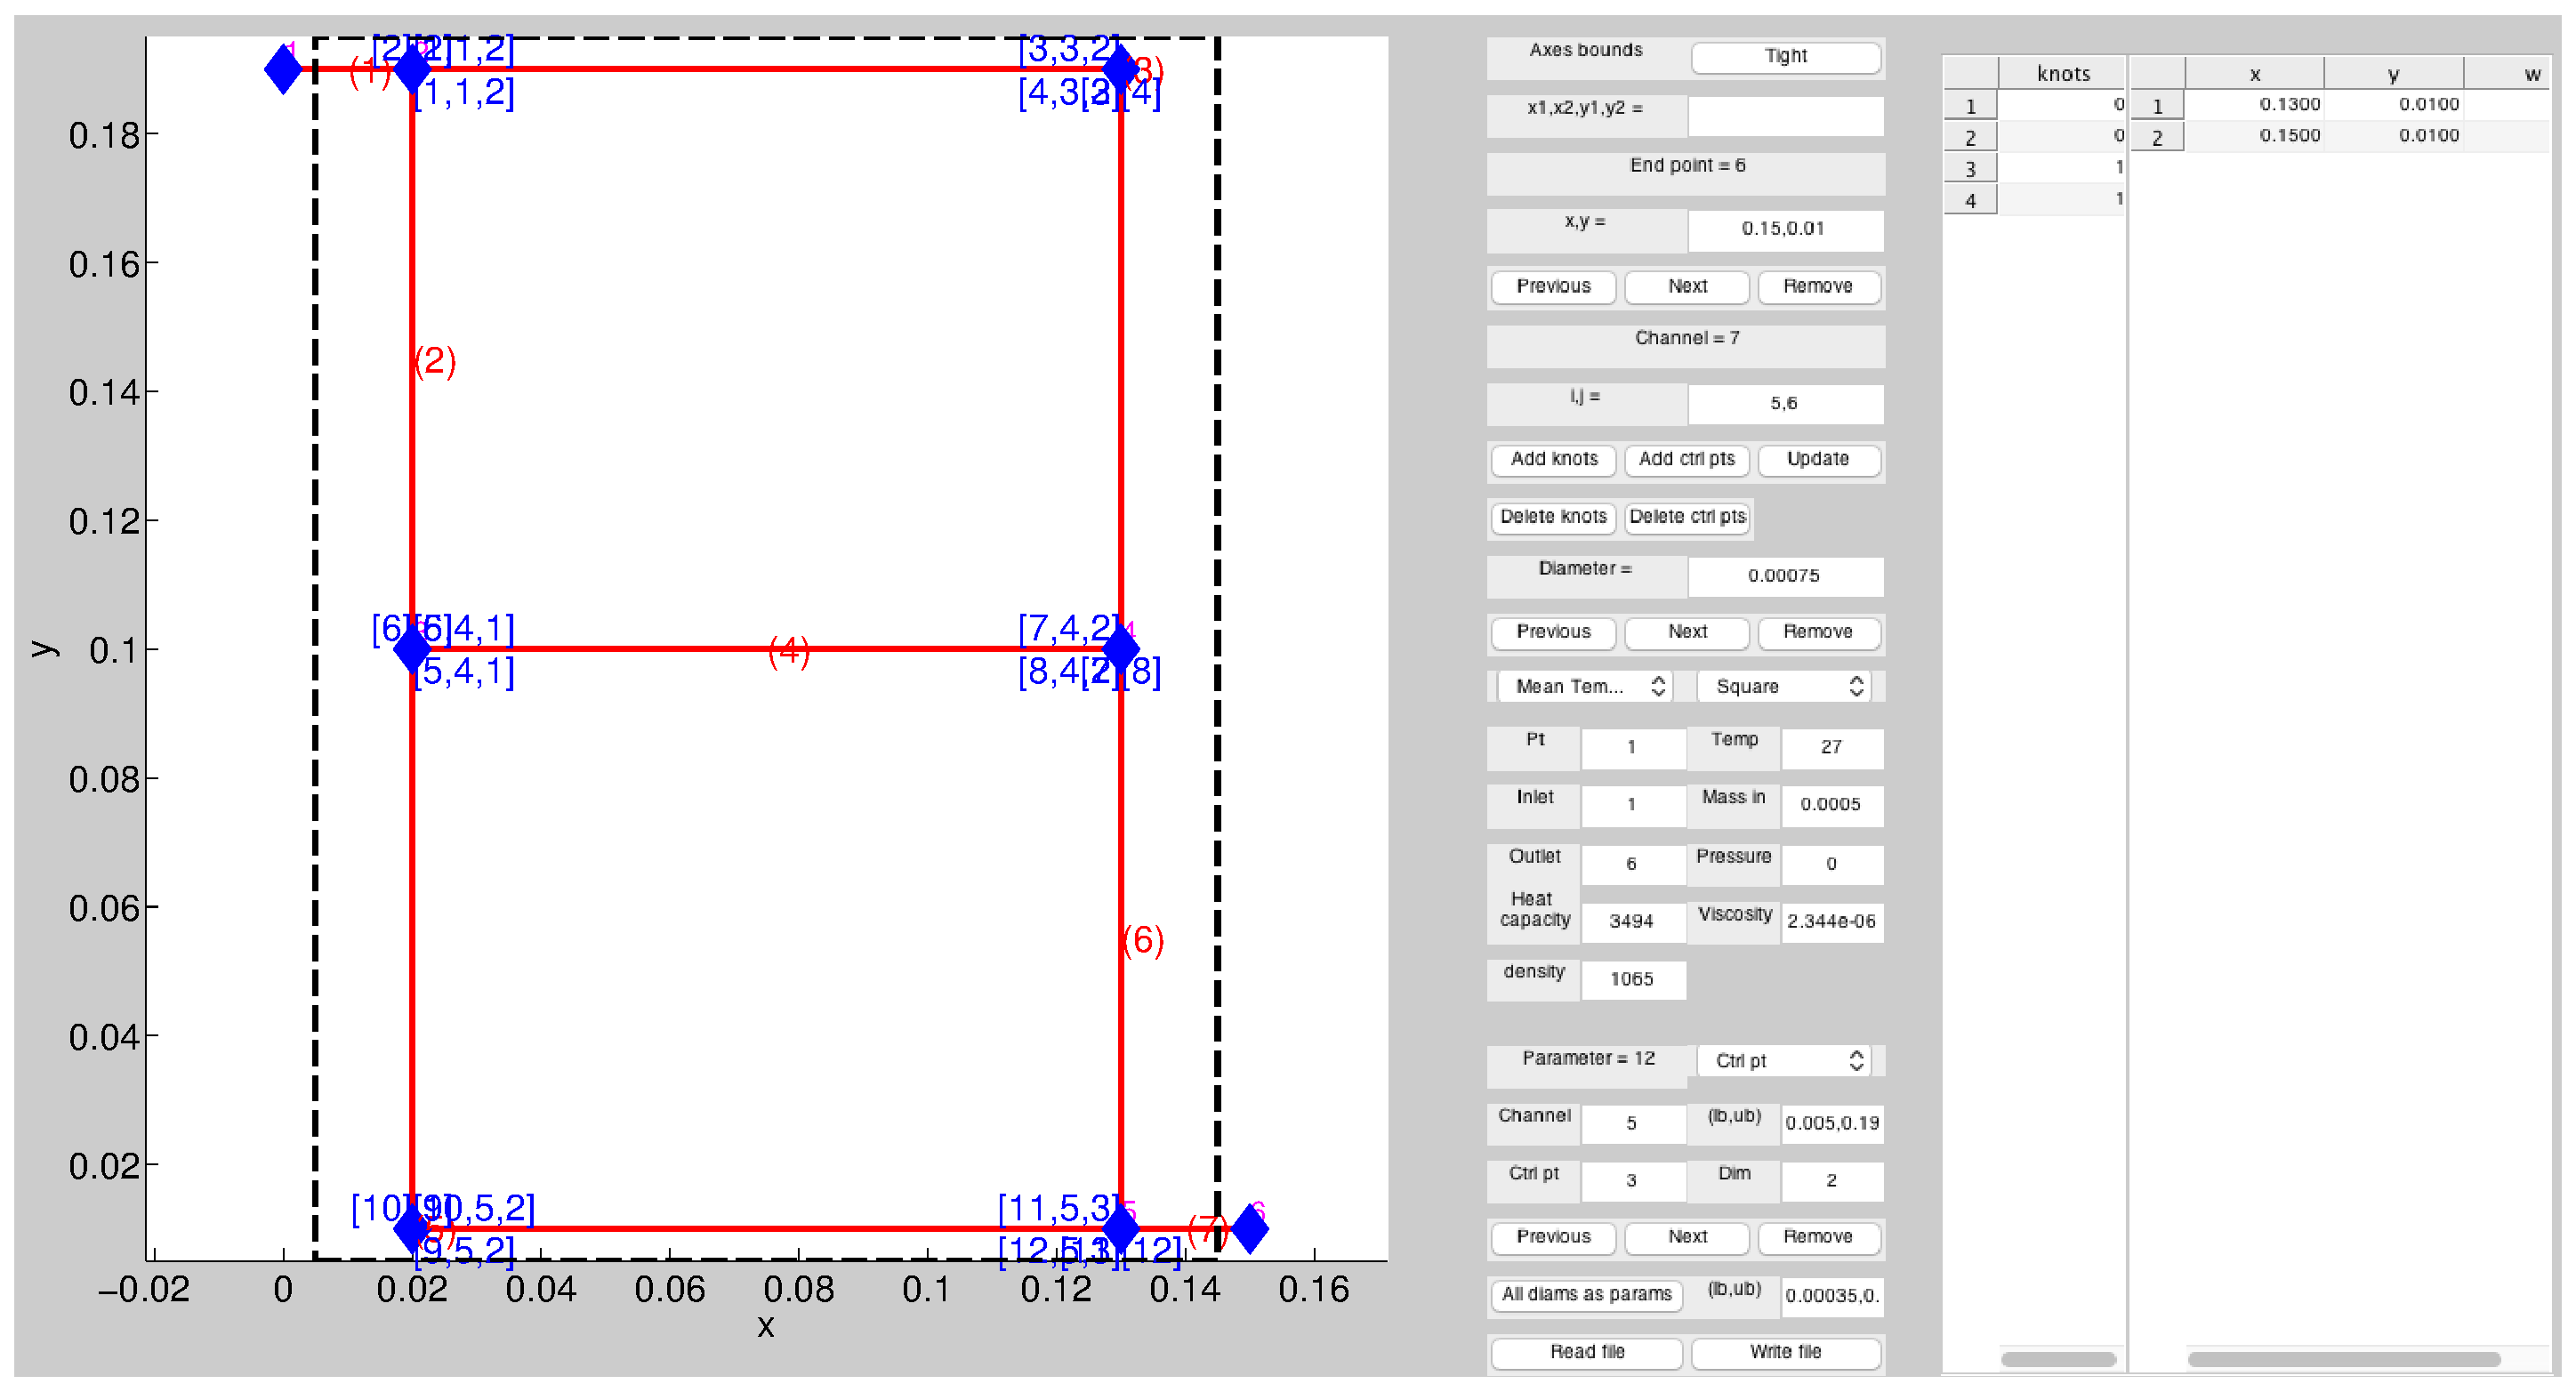
\includegraphics[width=\linewidth]{create_channel_gui_w_parallel2.eps}
\caption{Screenshot of GUI for creating channel. \label{fig_create_channel_gui}}
\end{figure}
A GUI tool \texttt{create\_channel\_gui.m} can be used to conveniently create channels. A screenshot of the creation of the 2-branch parallel network is shown in Fig.\ \ref{fig_create_channel_gui}. The left side shows the channels including the channel number, channel end point number and control points that are design parameters. The middle section consists of five parts. The first part ``Axes bounds'' allows the user to adjust the x-,y-axes limits and tighten the figure. The second part allows the user to create the channel end points, the connectivity of the channels and add/remove control points and change the knot vector of the channels. The control points and knot vector of a channel are listed in the right most columns. 

The properties of the flow, the type of simplified model, cross section of the channel etc can be changed in the third part. However, this part only allow the properties at one inlet/outlet to be specified. When multiple inlets/outlets are required, the network is first created with the flow properties etc specified for one of the inlets/outlets. After the channel file is created, open the file with a text editor and add the other inlet(s) following the single inlet specified below the keyword ``end point number and temperature''. Remember to change the number of inlets following the keyword. Additional outlets are specified with the keyword ``pressure out''. 

The design parameters are specified in the fourth part. Two types of design parameters are available: Ctrl pt (control point location) and diam (diameter). The design parameters are only used when optimization is run. Optimization is performed from a separate directory Opt-IGFEM-2D. The user manual for optimization can be found in that directory. 

The fifth part contains to buttons ``Read file'' and ``Write file''. The user is encouraged to open any of the channel files in the directory ChannelFiles to experiment with the GUI. It is also a good practice to save the channel file every now and then.
 
\FloatBarrier
\section{Examples}
\subsection{Example 1: Semicircular channel}
\label{subsec_semicircular_example}
\begin{figure}[!h]
\centering
\begin{subfigure}{0.55\textwidth}
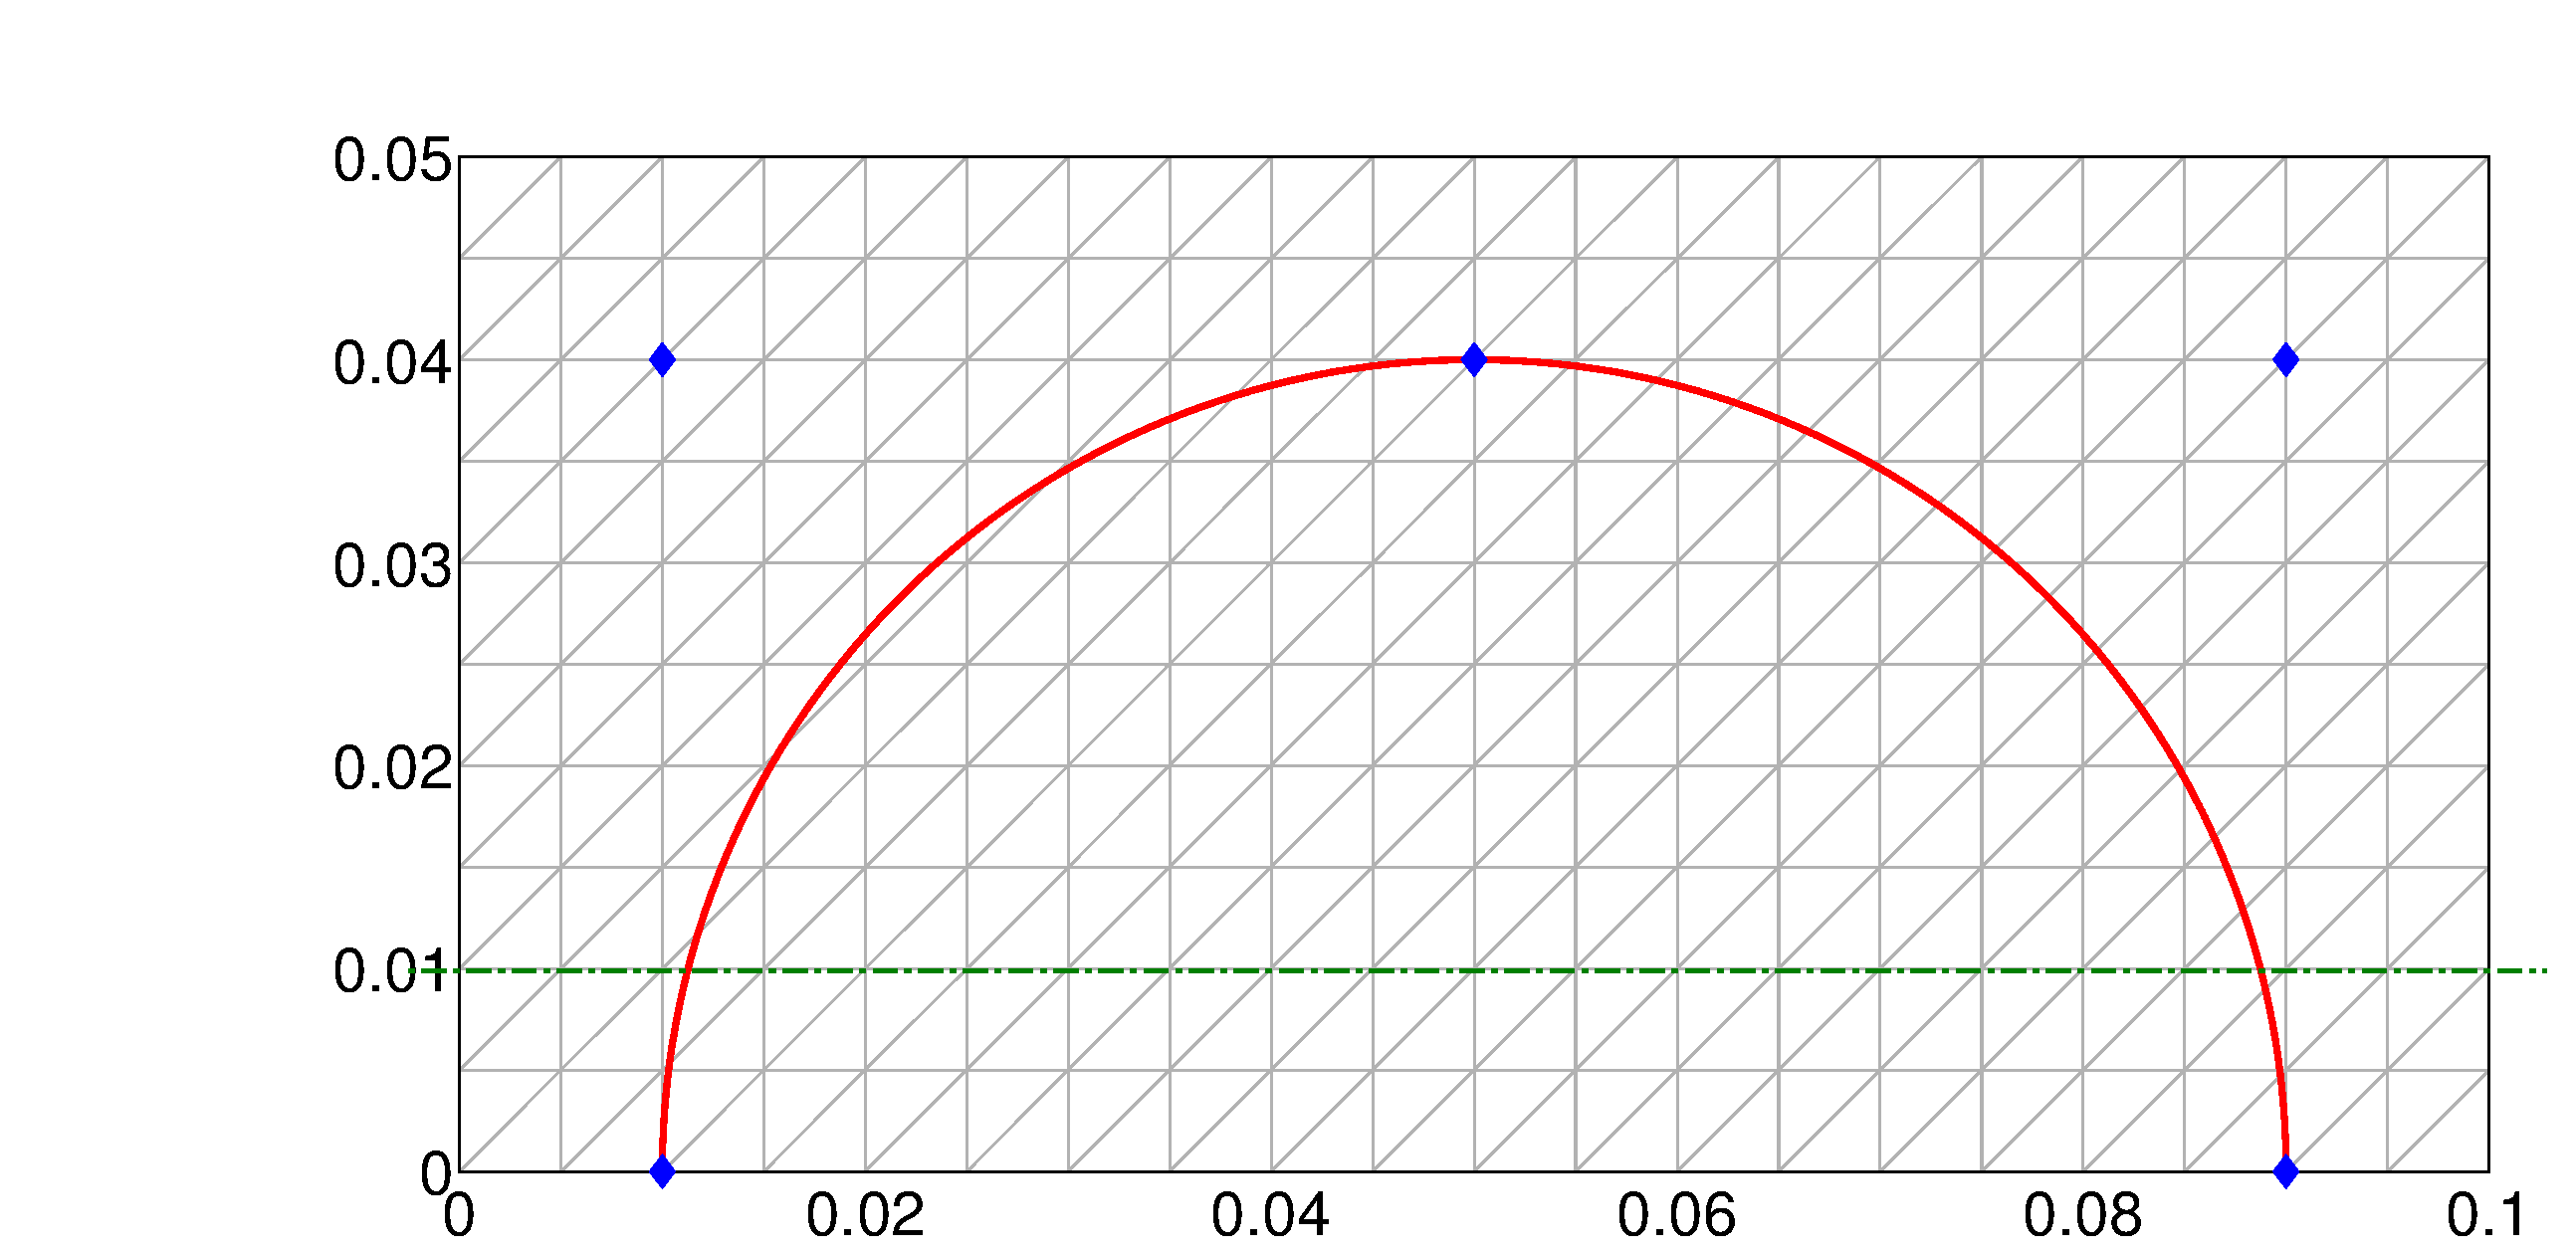
\includegraphics[width=\linewidth]{semicircular_channel_w_mesh.eps}
\caption{}
\end{subfigure}

\centering
\begin{subfigure}{0.5\textwidth}
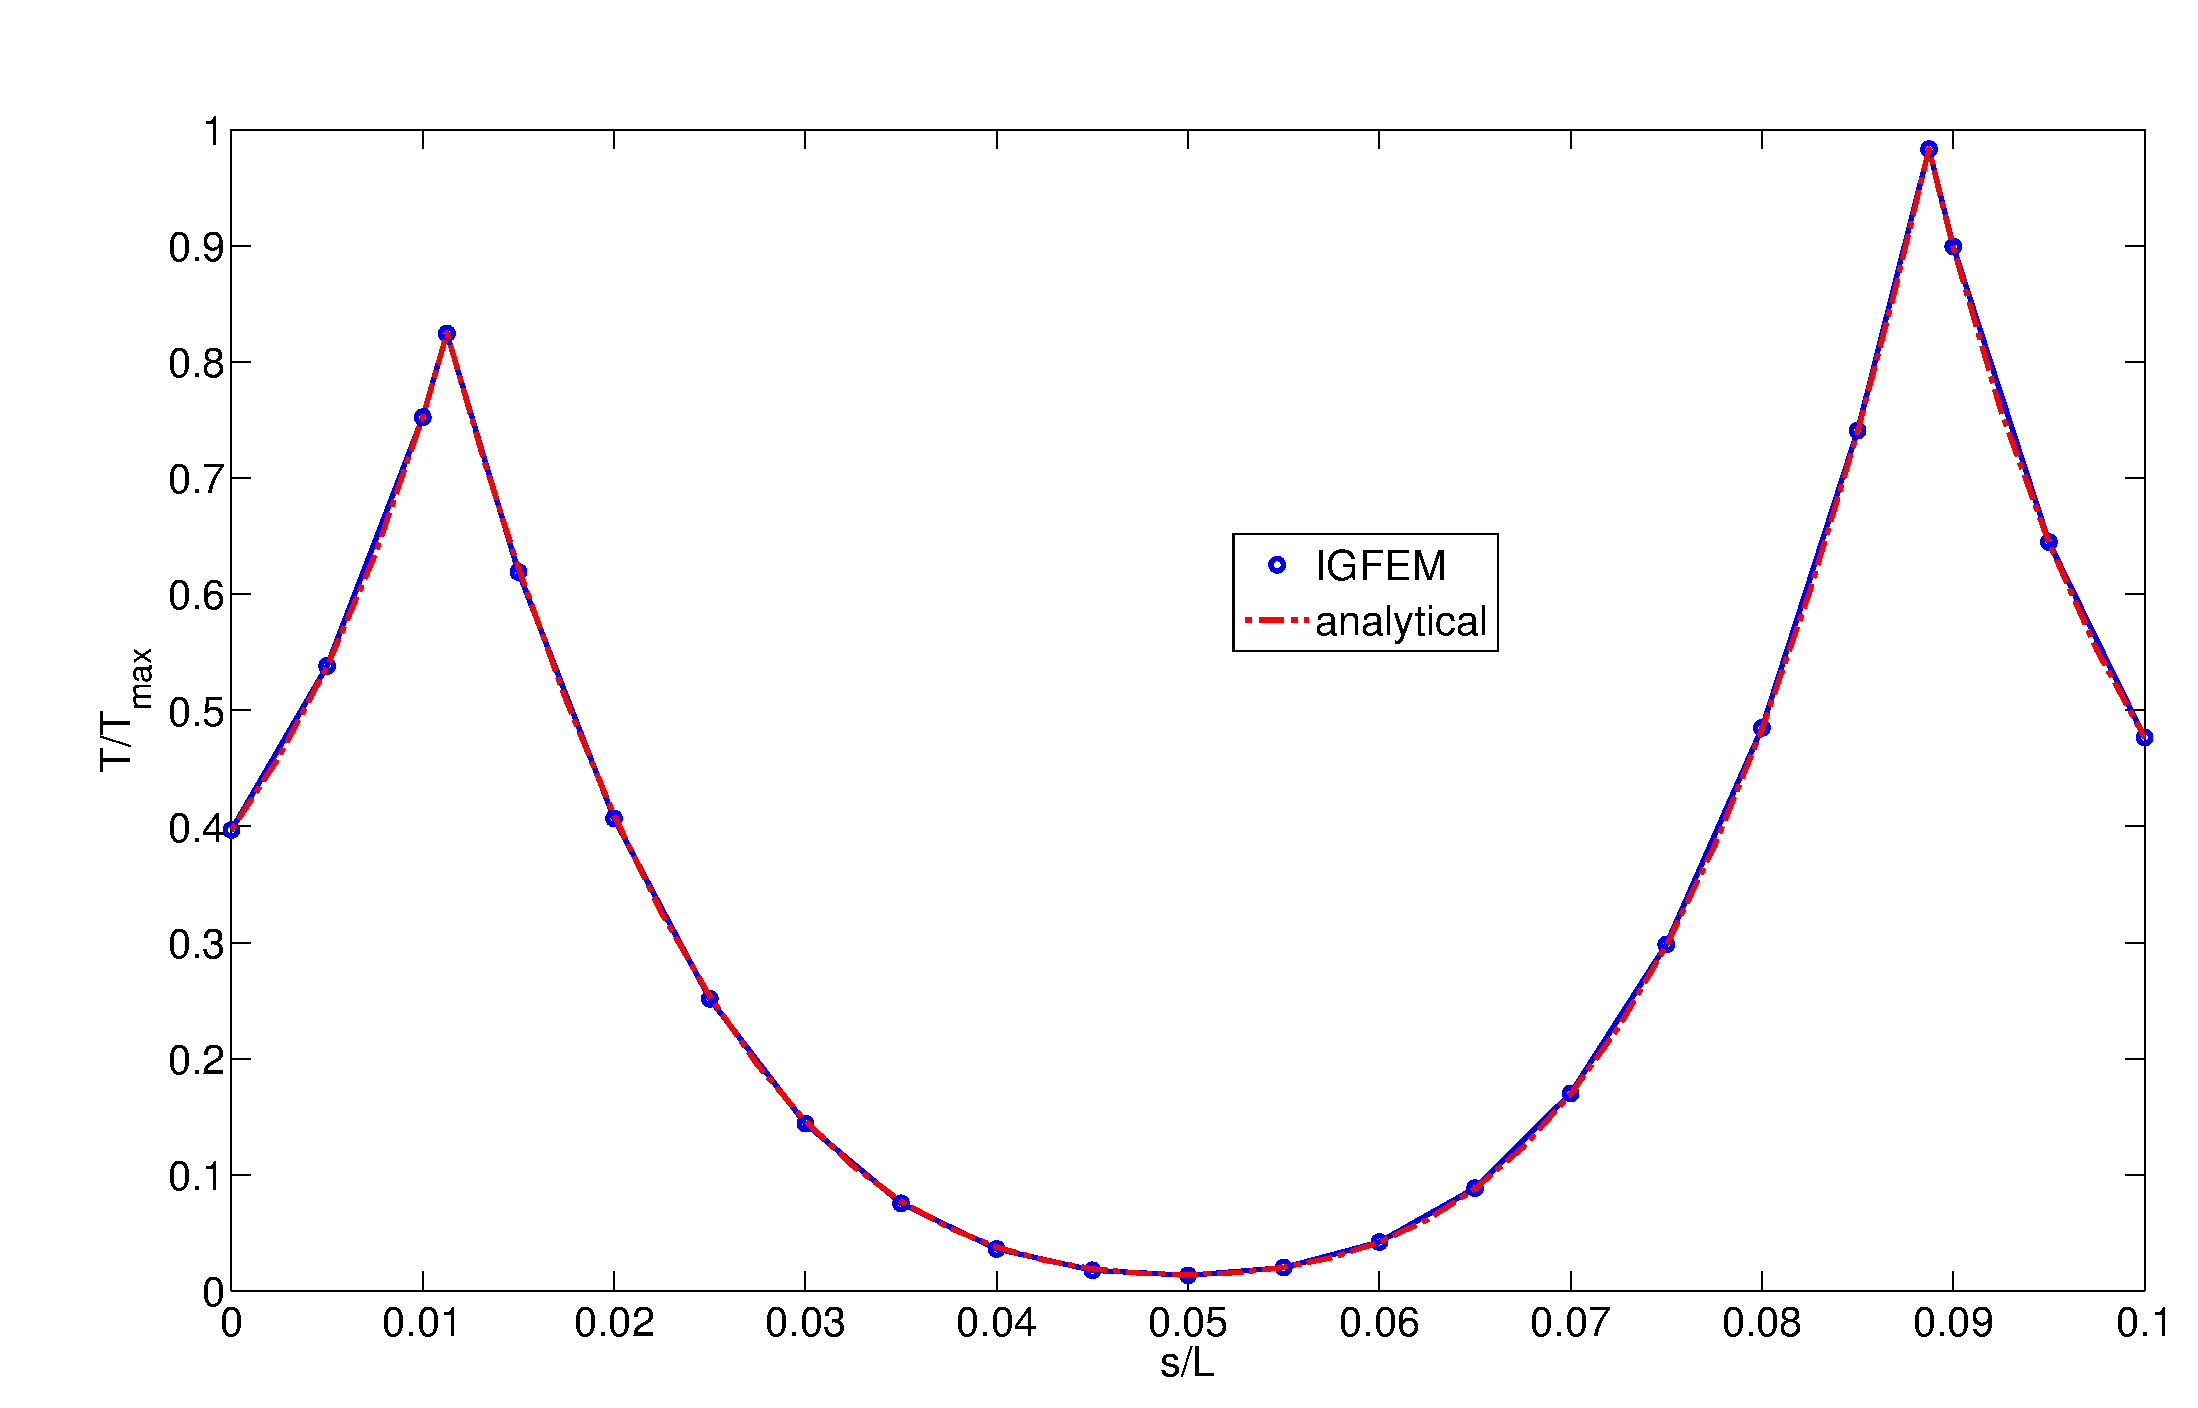
\includegraphics[width=\linewidth]{polyIGFEM_semicircular_T_vs_x_yp01.eps}
\caption{}
\end{subfigure}

\centering
\begin{subfigure}{0.5\textwidth}
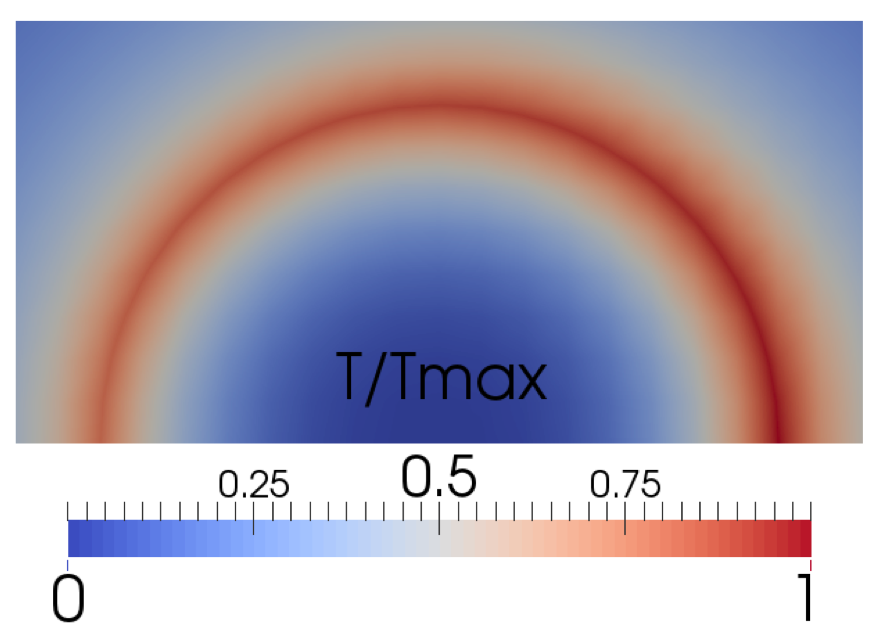
\includegraphics[width=\linewidth]{polynomial_IGFEM_semicircular_channel_T.png}
\caption{}
\end{subfigure}
\caption{(a) Structural mesh with 400 elements and a semicircular channel with its control points shown as blue diamonds. (b) The polynomial IGFEM and analytical solutions along the green dash-dot line in (a), i.e., along $y=0.01$. (c) The temperature distribution of the domain plotted with Paraview. \label{fig_semicircular}}
\end{figure}
The example here is used as a convergence study problem in \cite{Tan15}. We first run this example using polynomial IGFEM and the parameters mentioned in\cite{Tan15}. The distributed heat source consistent with the manufactured solution has to be applied in the file \texttt{body\_source\_functions.cpp} in the directory mx\texttt{\_}FEM. One can do that by uncommenting the \texttt{\#define SEMICIRCULAR\_CHANNEL} directive in the file. In addition, one must also uncomment the  \texttt{\#define source\_functions} directives in \texttt{compute\_IGFEM\_element.cpp} and   \texttt{compute\_regular\_element.cpp}. The analytical solution is defined in \texttt{analytical\_soln.m}.   The mesh used for this example, a comparison of the calculated temperature and the analytical solution, and the temperature distribution in the domain are shown in Fig.\ \ref{fig_semicircular}. The calculated errors in the $L^2$ and $H^1$ norms are respectively 5.1e-4 and 3.5e-1. Mesh method (ii) is used with the input variables in Table \ref{tab_semicircular_mesh_method2}. The remaining input variables are shown in Table \ref{tab_semicircular1} and \ref{tab_semicircular2}. 

We next run the example using NURBS-based IGFEM. This can be achieved simply by setting the variable \texttt{polyIGFEM} in Table \ref{tab_semicircular1} to \texttt{false}. The calculated errors in the $L^2$ and $H^1$ norms are respectively 4.6e-4 and 3.4e-1. The temperature plots are indistinguishable from those in Fig.\ \ref{fig_semicircular}. 

To use a conforming mesh, one needs to use mesh method (i). The Abaqus input files with conforming meshes for the semicircular channel of the particular radius are \texttt{conform1b\_temp\_all\_semicircle\_ro\_p04.inp}, \texttt{conform2\_temp\_all\_semicircle\_ro\_p04.inp} etc in the directory mesh\texttt{\_}conforming\texttt{\_}abaqus. The exploration of that method is left to the user. 

\FloatBarrier
 
\begin{table}[!h]
\caption{Mesh method (ii) variable for Sec.\ \ref{subsec_semicircular_example}.}
\label{tab_semicircular_mesh_method2}
\centering
\begin{tabular}{|c|c|}
\hline
Variable name & Value \\
\hline
\texttt{mesh.boundary.xi} & 0\\
\hline
\texttt{mesh.boundary.xf} & 0.1 \\
\hline
\texttt{mesh.boundary.yi} & 0 \\
\hline
\texttt{mesh.boundary.yf} & 0.05 \\
\hline
\texttt{meshSizes} & [20,10] \\
\hline
\texttt{mesh.elem.material} & \texttt{int32(ones(size(mesh.elem.elem\_node,1),1))} \\
\hline
\texttt{mesh.material.conductivity} & 1.0 \\
\hline
\texttt{mesh.elem.heatSource} & 0.0 \\
\hline
\end{tabular}
\end{table}

\begin{table}[!h]
\caption{Variables values for Sec.\ \ref{subsec_semicircular_example}. Variables with their values left blank are unused. }
\label{tab_semicircular1}
\centering
\begin{tabular}{|c|c|}
\hline
Variable name & Variable value\\
\hline
channelFile & \texttt{semicircle.channel}\\
\hline
\texttt{mesh.BCs.boundaries} & [1,2,3,4]\\
\hline
\texttt{mesh.BCs.types} & [1,1,1,1] \\
\hline
\texttt{mesh.BCs.values\_or\_funcs} & [u,u,u,u] where u = @(x,y) \texttt{analytical\_soln}(x,y) \\
\hline
\texttt{mesh.convect.coef} & 0\\
\hline
\texttt{mesh.convect.Tref} & 0 \\
\hline
\texttt{triNpt1D} & 4 (only used for polynomial IGFEM) \\
\hline
\texttt{triNpt2D} & 7 (only used for polynomial IGFEM)\\
\hline
\texttt{quaNpt1Dt} & 4 (only used for NURBS-based IGFEM) \\
\hline
\texttt{quaNpt1Dn} &  4 (only used for NURBS-based IGFEM) \\
\hline
\texttt{quadNpt1D} & \\
\hline
\texttt{polyIGFEM} & true\\
\hline
\texttt{supg} & false \\
\hline
\texttt{postProcessing} & true \\
\hline 
\texttt{outfile} & 'semicircularChannel' \\
\hline
\texttt{scalarname} & 'T' \\
\hline
\texttt{errorAnalysis} & true \\
\hline
\texttt{isAnalytical} & true. Need to define variable soln = @(x,y) \texttt{analytical\_soln}(x,y)\\
\hline
\texttt{isConformingMesh} & false \\
\hline
\end{tabular}
\end{table}

\begin{table}[!h]
\caption{Variables values for Sec.\ \ref{subsec_semicircular_example}. }

\label{tab_semicircular2}
\centering
\begin{tabular}{|c|c|}
\hline
\texttt{calcItrsectVel}  & false \\
\hline
\texttt{moveNode.distFrac} & \\ 
\hline
\texttt{moveNode.maxAttempts} &  \\
\hline
\texttt{moveNode.randDirection} & \\
\hline 
\texttt{tol.node} & \\
\hline
\texttt{tol.boundary} & 1e-13\\
\hline
\texttt{tol.nurbsParam} & 1e-8\\
\hline
\texttt{tol.epsco} & 1e-15\\
\hline
\texttt{tol.epsge} & 1e-6\\
\hline
\texttt{tol.cosAngleTol} & cos(20*pi/180.0)\\
\hline
\texttt{tol.halfLineWidthFrac} &  1e-4\\
\hline
\texttt{tol.vert} & \\
\hline
\texttt{tol.intersectEdges} & 1e-13\\
\hline
\texttt{opt.maxRefineLevel} & 0\\
\hline
\texttt{opt.refineJuncElem} & false\\
\hline
\texttt{slenderTol.minAngle} & 5\\
\hline
\texttt{slenderTol.maxAspectRatio} & inf\\
\hline
\end{tabular}
\end{table}

\FloatBarrier
\subsection{Example 2: Two-branch parallel network}
\label{subsec_parallelTwo_example}
\begin{figure}[!h]
\centering
\begin{subfigure}{0.28\textwidth}
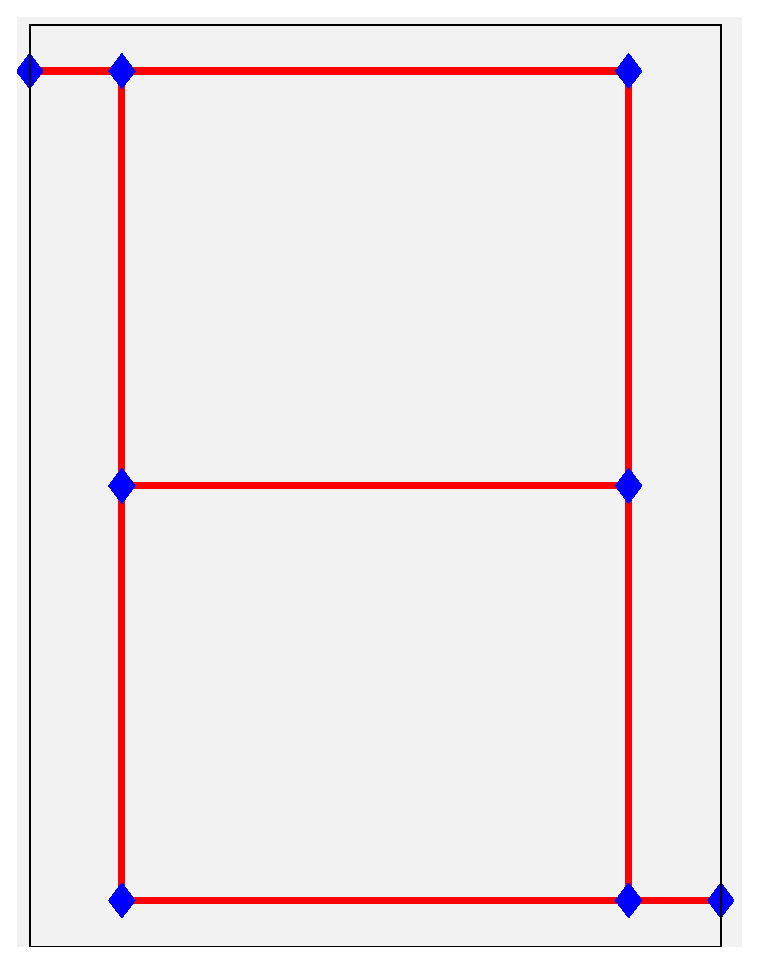
\includegraphics[width=\linewidth]{parallelTwoRef.eps}
\caption{}
\end{subfigure}
\begin{subfigure}{0.28\textwidth}
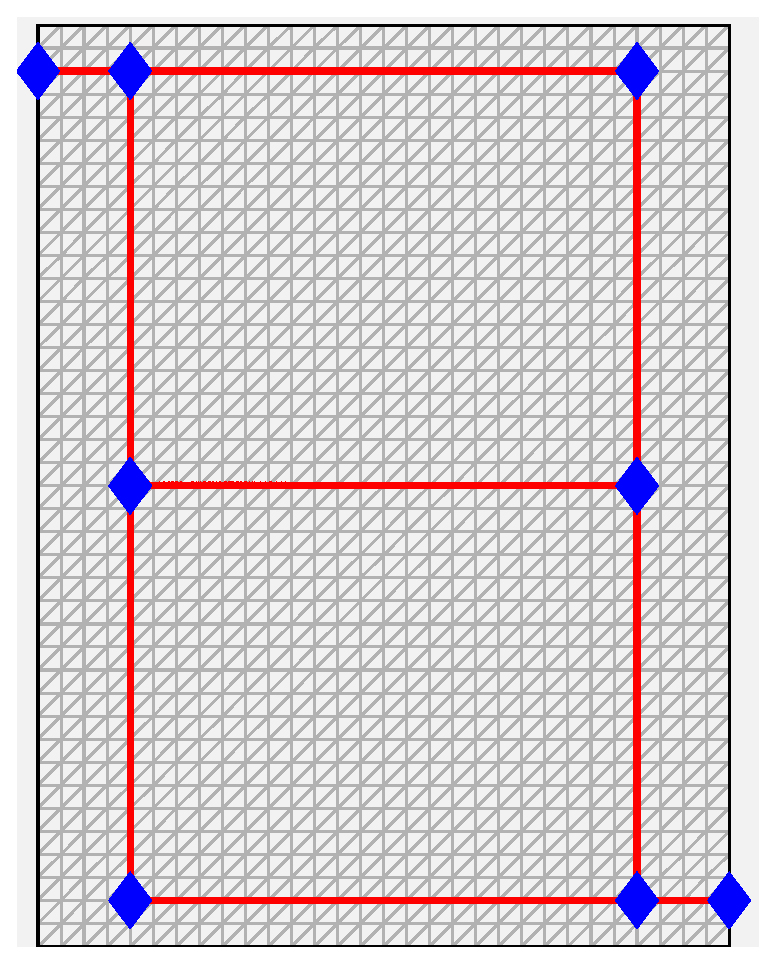
\includegraphics[width=\linewidth]{parallelTwo_reference_30x40_mesh.eps}
\caption{}
\end{subfigure}
\begin{subfigure}{0.35\textwidth}
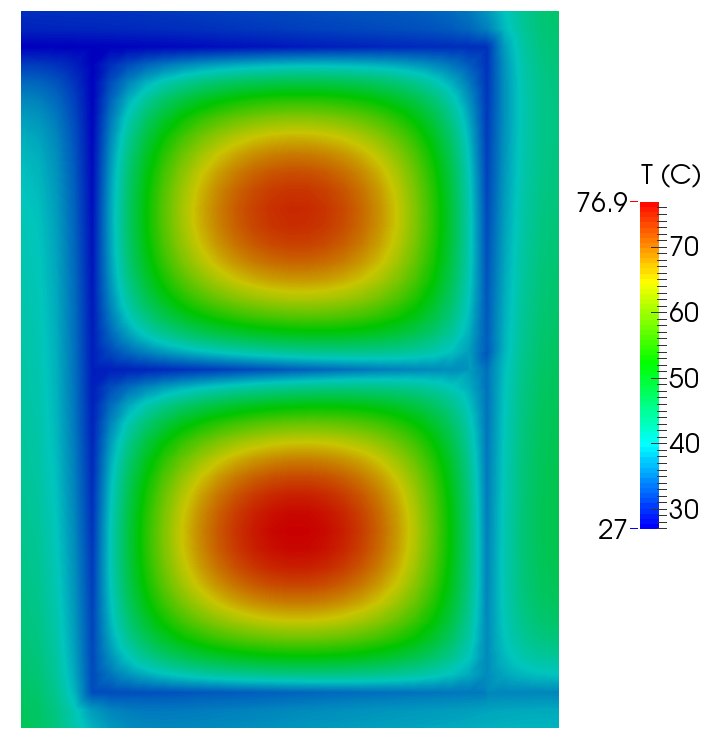
\includegraphics[width=\linewidth]{parallelTwoRefT.png}
\caption{}
\end{subfigure}
\caption{(a) Panel with embedded two-branch channel network, insulated boundaries, a uniform heat distribution of $500\,\mathrm{Wm^{-1}K^{-1}}$ and a coolant entering at 28.2 ml/min (0.5 g/s) and 23\degree C. (b) The non-conforming mesh used to obtain (c) the temperature distribution of the panel. \label{fig_parallelTwo}}
\end{figure}
In this example, we simulate the temperature in an insulated domain embedded with a two-branch parallel network shown in Fig.\   \ref{fig_parallelTwo}. The mesh is generated using mesh method (ii) with variable values presented in Table \ref{tab_parallelTwo_mesh_method2}. The other variable values are listed in Table \ref{tab_parallelTwo1} and \ref{tab_parallelTwo2} .

\begin{table}[!h]
\caption{Mesh method (ii) variable for Sec.\ \ref{subsec_parallelTwo_example}. SI units are used for all quantities except temperature, which is in \degree C.}
\label{tab_parallelTwo_mesh_method2}
\centering
\begin{tabular}{|c|c|}
\hline
Variable name & Value \\
\hline
\texttt{mesh.boundary.xi} & 0\\
\hline
\texttt{mesh.boundary.xf} & 0.15 \\
\hline
\texttt{mesh.boundary.yi} & 0 \\
\hline
\texttt{mesh.boundary.yf} & 0.2 \\
\hline
\texttt{meshSizes} & [40,30] \\
\hline
\texttt{mesh.elem.material} & \texttt{int32(ones(size(mesh.elem.elem\_node,1),1))} \\
\hline
\texttt{mesh.material.conductivity} & 2.7*0.003 \\
\hline
\texttt{mesh.elem.heatSource} & 500.0 \\
\hline
\end{tabular}
\end{table}

\begin{table}[!h]
\caption{Variables values for Sec.\ \ref{subsec_parallelTwo_example}. Variables with their values left blank are unused.}
\label{tab_parallelTwo1}
\centering
\begin{tabular}{|c|c|}
\hline
Variable name & Variable value\\
\hline
channelFile & \texttt{parallel2\_start.channel}\\
\hline
\texttt{mesh.BCs.boundaries} & [ ]\\
\hline
\texttt{mesh.BCs.types} &  \\
\hline
\texttt{mesh.BCs.values\_or\_funcs} & \\
\hline
\texttt{mesh.convect.coef} & 0\\
\hline
\texttt{mesh.convect.Tref} & 0 \\
\hline
\texttt{triNpt1D} & 4\\
\hline
\texttt{triNpt2D} & 7 \\
\hline
\texttt{quaNpt1Dt} & \\
\hline
\texttt{quaNpt1Dn} & \\
\hline
\texttt{quadNpt1D} & \\
\hline
\texttt{polyIGFEM} & true\\
\hline
\texttt{supg} & true \\
\hline
\texttt{postProcessing} & false \\
\hline 
\texttt{outfile} & 'parallelTwo' \\
\hline
\texttt{scalarname} & 'T' \\
\hline
\texttt{errorAnalysis} & false \\
\hline
\texttt{isAnalytical} & false\\
\hline
\texttt{isConformingMesh} & false \\
\hline
\end{tabular}
\end{table}

\begin{table}[!h]
\caption{Variables values for Sec.\ \ref{subsec_parallelTwo_example}. }

\label{tab_parallelTwo2}
\centering
\begin{tabular}{|c|c|}
\hline
\texttt{calcItrsectVel}  & false \\
\hline
\texttt{moveNode.distFrac} & \\ 
\hline
\texttt{moveNode.maxAttempts} &  \\
\hline
\texttt{moveNode.randDirection} & \\
\hline 
\texttt{tol.node} & \\
\hline
\texttt{tol.boundary} & 1e-13\\
\hline
\texttt{tol.nurbsParam} & 1e-8\\
\hline
\texttt{tol.epsco} & 1e-15\\
\hline
\texttt{tol.epsge} & 1e-6\\
\hline
\texttt{tol.cosAngleTol} & cos(20*pi/180.0)\\
\hline
\texttt{tol.halfLineWidthFrac} &  1e-4\\
\hline
\texttt{tol.vert} & \\
\hline
\texttt{tol.intersectEdges} & 1e-13\\
\hline
\texttt{opt.maxRefineLevel} & 0\\
\hline
\texttt{opt.refineJuncElem} & false\\
\hline
\texttt{slenderTol.minAngle} & 5\\
\hline
\texttt{slenderTol.maxAspectRatio} & inf\\
\hline
\end{tabular}
\end{table}

\FloatBarrier
\section{References}
\bibliographystyle{plainnat}
\bibliography{references}    
\end{document}
